\documentclass{article}
    \usepackage{ctex}
    \usepackage[margin = 2cm]{geometry}
    \usepackage{amsthm}
    \usepackage{amsfonts}
    \usepackage{amsmath}
    \usepackage{amssymb}
    \usepackage{wrapfig}
    \usepackage{subfigure}
    \usepackage{tikz}
    \usetikzlibrary{calc}
    \usetikzlibrary{intersections} 
    \newtheorem{QUESTION}{问题}
    \newenvironment{SOLUTION}[1][{}]{{\noindent\heiti 解#1:}}{\hfill $\square$\par} 
    \newcommand{\Ln}{\mathrm{Ln}}
    \title{复变思考题解答}
    \author{自64\qquad 赵文亮\qquad 2016011452\thanks{zhaowl16@mails.tsinghua.edu.cn}}
    \begin{document}
    \maketitle
    \begin{QUESTION}
    设分式线性变换
    \begin{equation}
    \omega = \frac{az+b}{cz+d}
    \label{equ:mobius}
    \end{equation}
    其中$a,b,c,d\in\mathbb{R}$且$ad-bc\neq 0$。
    则式~\eqref{equ:mobius}~保广义圆,且对于圆$z=z_0+re^{i\theta}$,变换后为$\omega = \omega_0+Re^{i\varphi }$,求$\omega_0,R,\varphi$的表达式。
    \end{QUESTION}
    
    \begin{SOLUTION}
    由已知$a,c$不同时为0。
    $ac\neq 0$时,分式线性变换~\eqref{equ:mobius}~可以写成
    \begin{equation}
    \omega = \dfrac{az+b}{cz+d}=\dfrac{a}{c}\cdot\dfrac{z+\dfrac{b}{a}}{z+\dfrac{d}{c}}=\dfrac{a}{c}\left(1+\dfrac{\dfrac{b}{a}-\dfrac{d}{c}}{z+\dfrac{d}{c}}\right)
    \label{equ:transform}
    \end{equation}
    $a=0,c\neq 0$时,分式线性变换~\eqref{equ:mobius}~可以写成
    \begin{equation}
        \tag{\ref{equ:transform}$'$}
        \omega = \dfrac{b}{c}\cdot\dfrac{1}{z+\dfrac{d}{c}}
        \label{equ:transform'}
    \end{equation}
    $a\neq 0, c=0$时,分式线性变换~\eqref{equ:mobius}~可以写成
    \begin{equation}
        \tag{\ref{equ:transform}$''$}
        \omega = \dfrac{a}{d}z+\dfrac{b}{d}
        \label{equ:transform''}
    \end{equation}
    即总可以将\eqref{equ:mobius}看成三种变换的复合:平移变换、倒数变换、放缩变换。下面对于圆$z=z_0+re^{i\theta}$在每种变换作用后的结果分别分析。
    \begin{enumerate}
    \item 平移变换
    \begin{equation}
    \omega_1 = z+z_{\rm m}
    \end{equation}
    对于圆$z=z_0+re^{i\theta}$,变换后易得
    \begin{equation}
    \omega_1=z_0+z_m+re^{i\theta}\triangleq \omega_0+Re^{i\varphi}
    \end{equation}
    即对于平移变换,易得
    \begin{equation}
    \begin{cases}
    \omega_0 =z_0+z_m\\
    R = r\\
    \varphi  = \theta+2k\pi\qquad(k\in\mathbb{Z})
    \end{cases}
    \label{equ:move}
    \end{equation}
    \item 放缩变换
    \begin{equation}
    \omega_2 = sz
    \end{equation}
    其中$s\in \mathbb{R}$为放缩系数。则经放缩变换后
    \begin{equation}
    \omega_2 = s(z_0+re^{i\theta})=sz_0+sre^{i\theta}\triangleq \omega_0+Re^{i\varphi}
    \end{equation}
    即
    \begin{equation}
    \begin{cases}
    w_0=sz_0\\
    R=|s|r\\
    \varphi = \theta+\arg s +2k\pi\qquad(k\in\mathbb{Z})
    \end{cases}
    \label{equ:scale}
    \end{equation}
    \item 倒数变换
    \begin{equation}
    \omega_3 = \frac{1}{z}
    \label{equ:reciprocal}
    \end{equation}
    考虑复平面上圆的一般形式
    \begin{equation}
    z\bar{z}+\bar{\alpha}z+\alpha \bar{z}+\beta=0
    \label{equ:circle}
    \end{equation}
    不难推出式~\eqref{equ:circle}~对应的圆心和半径为:
    \begin{equation}
    \begin{cases}
    z_0=-\alpha\\
    r=\sqrt[]{|\alpha|^2-\beta}
    \end{cases}
    \end{equation}
    下面进行式~\eqref{equ:reciprocal}~的变换,可以得到
    \begin{equation*}
    \frac{1}{\omega_3\overline{\omega_3}}+\bar{\alpha}\frac{1}{\omega_3}+\alpha\frac{1}{\overline{\omega_3}}+\beta=0
    \end{equation*}
    或
    \begin{equation}
    \beta\omega_3\overline{\omega_3}+\bar{\alpha}\overline{\omega_3}+\alpha\omega_3+1=0
    \end{equation}
    当$\beta=0$(即$|z_0|=r$)时,上式退化为直线;$\beta\neq 0$时,上式改写为:
    \begin{equation}
    \omega_3\overline{\omega_3}+\frac{\bar{\alpha}}{\beta}\overline{\omega_3}+\frac{\alpha}{\beta}\omega_3+\frac{1}{\beta}=0
    \label{equ:omega_circle}
    \end{equation}
    对比式~\eqref{equ:circle}~,可知式~\eqref{equ:omega_circle}~也表示一个圆,且有
    \begin{equation}
    \begin{cases}
    \omega_0=-\dfrac{\bar{\alpha}}{\beta}=\dfrac{\overline{z_0}}{|z_0|^2-r^2}\\[3ex]
    R=\sqrt[]{\dfrac{|\alpha|^2}{\beta^2}-\dfrac{1}{\beta}}=\dfrac{r}{|\beta|}=\dfrac{r}{\left||z_0|^2-r^2\right|}
    \end{cases}
    \end{equation}
    
    \begin{equation}
    \omega_3=\dfrac{1}{z_0+re^{i\theta}}=\omega_0+Re^{i\varphi}
    \end{equation}
    将已经求得的$\omega_0$和$R$的表达式代入求解$e^{i\varphi}$。先考虑$|z_0|^2-r^2>0$的情况:
    \begin{equation}
    \begin{split}
    e^{i\varphi}&=\dfrac{\omega_3-\omega_0}{R}=\dfrac{\dfrac{1}{z_0+re^{i\theta}}-\dfrac{\overline{z_0}}{|z_0|^2-r^2}}{\dfrac{r}{|z_0|^2-r^2}}\\[2ex]
    &=-\dfrac{r+\overline{z_0}e^{i\theta}}{z_0+re^{i\theta}}
    \end{split}
    \label{equ:varphi}
    \end{equation}
 
 
    下面说明,$\forall \varphi,\exists !\theta\in[0,2\pi), s.t.$
    \begin{equation*}
    e^{i\varphi}=-\dfrac{r+\overline{z_0}e^{i\theta}}{z_0+re^{i\theta}}
    \end{equation*}
    事实上,由上式等价于
    \begin{equation}
    e^{i\theta}=-\dfrac{r+z_0e^{i\varphi}}{\overline{z_0}+re^{i\varphi}}
    \label{equ:theta}
    \end{equation}
    计算等号右边的模方:
    \begin{equation}
    \begin{split}
    \left|
    -\dfrac{r+z_0e^{i\varphi}}{\overline{z_0}+re^{i\varphi}}\right|^2&=\dfrac{(r+z_0e^{i\varphi})(r+\overline{z_0}e^{-i\varphi})}{(\overline{z_0}+re^{i\varphi})(z_0+re^{-i\varphi})}\\
    &=\dfrac{r^2+r\overline{z_0}e^{-i\varphi}+rz_0e^{i\varphi}+|z_0|^2}{|z_0|^2+\overline{z_0}re^{-i\varphi}+z_0re^{i\varphi}+r^2}\\
    &=1
    \end{split}
    \end{equation}
    
    则式~\eqref{equ:theta}~必有解
    \begin{equation}
    \begin{split}
    \theta &= \frac{1}{i}\Ln\left(-\dfrac{r+z_0e^{i\varphi}}{\overline{z_0}+re^{i\varphi}}\right)\\
    &=\frac{1}{i}\left(\ln\left|-\dfrac{r+z_0e^{i\varphi}}{\overline{z_0}+re^{i\varphi}}\right|+i\arg \left(-\dfrac{r+z_0e^{i\varphi}}{\overline{z_0}+re^{i\varphi}}\right)+2k\pi i\right)\\
    &=\arg \left(-\dfrac{r+z_0e^{i\varphi}}{\overline{z_0}+re^{i\varphi}}\right)+2k\pi\qquad (k\in \mathbb{Z}) 
    \end{split}
    \end{equation}
    如果\textit{限定}$\theta\in [0,2\pi)$,则当$e^{i\varphi}$取定后,由上式可以解出\textit{唯一}的值。至此,我们已经可以得出,若$\theta$在$[0,2\pi)$变化,$\theta$从0增大到$2\pi $时,$e^{i\varphi}$这一复数也恰好绕单位圆走过了一圈,且不存在同一个$e^{i\varphi}$值对应$[0,2\pi)$中的两个或两个以上$\theta$值的情况。
    
    进一步可以求出$\varphi$的值。不难发现式~\eqref{equ:varphi}~和式~\eqref{equ:theta}~之间存在对称性。类似可以求得:
    \begin{equation}
    \varphi = 
    \arg \left(-\dfrac{r+\overline{z_0}e^{i\theta}}{z_0+re^{i\theta}}\right)+2k\pi\qquad (k\in \mathbb{Z}) 
    \label{rec:phi}
    \end{equation}
    若$|z_0|^2<r^2$,则
    $$R=\dfrac{r}{r^2-|z_0|^2}$$
    使用完全相同的推导方式(事实上只相差一个符号),可以得出
    \begin{equation}
        \tag{\ref{equ:varphi}$'$}
        e^{i\varphi}=\dfrac{r+\overline{z_0}e^{i\theta}}{z_0+re^{i\theta}}
        \label{equ:varphip}
        \end{equation}


        同理可证$\theta$从0增大到$2\pi$时,$e^{i\varphi}$恰好绕单位圆走过一圈。由式~\eqref{equ:varphip}~解出$\varphi$:
        \begin{equation}
            \tag{\ref{rec:phi}$'$}
            \varphi =
            \arg \left(\dfrac{r+\overline{z_0}e^{i\theta}}{z_0+re^{i\theta}}\right)+2k\pi\qquad (k\in \mathbb{Z})\label{rec:phi'}
            \end{equation}
    故可以得出结论,倒数变换将完整的圆映成完整的圆(或直线)。像为圆时($r\neq |z_0|$),将上述结果整理:
    \begin{equation}
    \begin{cases}
    \omega_0=\dfrac{\overline{z_0}}{|z_0|^2-r^2}\\[3ex]
    R=\dfrac{r}{||z_0|^2-r^2|}\\[3ex]
    \varphi = 
    \arg \left((r-|z_0|)\dfrac{r+\overline{z_0}e^{i\theta}}{z_0+re^{i\theta}}\right)+2k\pi\qquad (k\in \mathbb{Z}) 
    \end{cases}
    \label{equ:reciprocal}
    \end{equation}
    上式巧妙地利用因子$(r-|z_0|)$来实现符号的控制。

    \end{enumerate}
    至此,我们已经推导出来三种特殊的分式线性变换下圆心、半径、辐角的变换关系。下面利用式~\eqref{equ:move}\eqref{equ:scale}\eqref{equ:reciprocal}~求解一般的分式线性变换下三者的变换关系。
    \begin{itemize}
        \item $ac\neq 0$,如式~\eqref{equ:transform}~所示。首先进行平移操作$$z_1=z+\frac{d}{c}$$则
    \begin{equation}
    \begin{cases}
    z_{10}=z_0+\dfrac{d}{c}\\
    r_1=r\\
    \theta_1=\theta+2k\pi\qquad (k\in \mathbb{Z})
    \end{cases}
    \end{equation}
    再进行倒数变换$$z_2=\dfrac{1}{z_1}$$
    则
    \begin{equation}
    \begin{cases}
    z_{20}=\dfrac{\overline{z_{10}}}{|z_{10}|^2-r_1^2}=\dfrac{\overline{z_0}+\dfrac{d}{c}}{\left|z_0+\dfrac{d}{c}\right|^2-r^2}
    \\[2ex]
    r_2=\dfrac{r_1}{||z_{10}|^2-r_1^2|}=\dfrac{r}{\left|\left|z_0+\dfrac{d}{c}\right|^2-r^2\right|}\\[3ex]
    \begin{split}
    \theta_2&=\arg \left((r_1-|z_{10}|)\cdot\dfrac{r_1+\overline{z_{10}}e^{i\theta_1}}{z_{10}+r_1e^{i\theta_1}}\right)+2k\pi\\[2ex]
    &=\arg \left(\left(r-\left|z_0+\dfrac{d}{c}\right|\right)\cdot\dfrac{r+\left(\overline{z_0}+\dfrac{d}{c}\right)e^{i\theta}}{z_0+\dfrac{d}{c}+re^{i\theta}}\right)+2k\pi\qquad (k\in \mathbb{Z})
    \end{split}
    \end{cases}
    \label{equ:move_rec}
    \end{equation}
    再进行放缩变换$$z_3=\left(\frac{b}{a}-\frac{d}{c}\right)z_2$$
    则
    \begin{equation}
    \begin{cases}
    z_{30}=\left(\dfrac{b}{a}-\dfrac{d}{c}\right)z_{20}=\left(\dfrac{b}{a}-\dfrac{d}{c}\right)\dfrac{\overline{z_0}+\dfrac{d}{c}}{\left|z_0+\dfrac{d}{c}\right|^2-r^2}\\[2ex]
    r_3=\left|\dfrac{b}{a}-\dfrac{d}{c}\right|r_2=\left|\dfrac{b}{a}-\dfrac{d}{c}\right|\dfrac{r}{\left|\left|z_0+\dfrac{d}{c}\right|^2-r^2\right|}\\[2ex]
    \begin{split}
        \theta_3&=\theta_2+\arg\left(\dfrac{b}{a}-\dfrac{d}{c}\right)+2k\pi\\
        &=\arg \left(\left(\dfrac{b}{a}-\dfrac{d}{c}\right)\left(r-\left|z_0+\dfrac{d}{c}\right|\right)\dfrac{r+\left(\overline{z_0}+\dfrac{d}{c}\right)e^{i\theta}}{z_0+\dfrac{d}{c}+re^{i\theta}}\right)+2k\pi\qquad (k\in \mathbb{Z})  
    \end{split}
    \end{cases}
    \end{equation}
    再进行平移变换$z_4=z_3+1$,则
    \begin{equation}
    \begin{cases}
    z_{40} =z_{30}+1=\left(\dfrac{b}{a}-\dfrac{d}{c}\right)\dfrac{\overline{z_0}+\dfrac{d}{c}}{\left|z_0+\dfrac{d}{c}\right|^2-r^2}+1\\
    r_4 = r_3=\left|\dfrac{b}{a}-\dfrac{d}{c}\right|\dfrac{r}{\left|\left|z_0+\dfrac{d}{c}\right|^2-r^2\right|}\\
    \begin{split}
        \theta_4  &= \theta_3+2k\pi\\
        &=\arg \left(\left(\dfrac{b}{a}-\dfrac{d}{c}\right)\left(r-\left|z_0+\dfrac{d}{c}\right|\right)\dfrac{r+\left(\overline{z_0}+\dfrac{d}{c}\right)e^{i\theta}}{z_0+\dfrac{d}{c}+re^{i\theta}}\right)+2k\pi \qquad(k\in\mathbb{Z})   
    \end{split}
    \end{cases}
    \end{equation}
    最后进行放缩变换$z_5=\dfrac{a}{c}z_4$,则
    \begin{equation}
    \begin{cases}
    z_{50}=\dfrac{a}{c}z_{40}=\dfrac{a}{c}\left(\left(\dfrac{b}{a}-\dfrac{d}{c}\right)\dfrac{\overline{z_0}+\dfrac{d}{c}}{\left|z_0+\dfrac{d}{c}\right|^2-r^2}+1\right)\\[2ex]
    r_5 = \left|\dfrac{a}{c}\right|r_4=\dfrac{|bc-ad|}{c^2}\cdot\dfrac{r}{\left|\left|z_0+\dfrac{d}{c}\right|^2-r^2\right|}\\[2ex]
    \begin{split}
        \theta_5&=\theta_4+\arg\left(\dfrac{a}{c}\right)+2k\pi\\& = \arg \left(\left(\dfrac{a}{c}\right)\left(\dfrac{b}{a}-\dfrac{d}{c}\right)\left(r-\left|z_0+\dfrac{d}{c}\right|\right)\dfrac{r+\left(\overline{z_0}+\dfrac{d}{c}\right)e^{i\theta}}{z_0+\dfrac{d}{c}+re^{i\theta}}\right)+2k\pi\\
        &= \arg \left((bc-ad)\left(r-\left|z_0+\dfrac{d}{c}\right|\right)\dfrac{r+\left(\overline{z_0}+\dfrac{d}{c}\right)e^{i\theta}}{z_0+\dfrac{d}{c}+re^{i\theta}}\right)+2k\pi\qquad(k\in\mathbb{Z})
    \end{split} 
    \end{cases}
    \label{ans:1}
    \end{equation}

    $z_{50},r_5,\theta_5$为所求。

    \item $a=0,c\neq 0$,如式~\eqref{equ:transform'}~所示。同样进行平移变换和倒数变换,结果同式~\eqref{equ:move_rec}~。再进行放缩变换
    $$z_3=\dfrac{b}{c}z_2$$
    可得:
    \begin{equation}
        \begin{cases}
        z_{30}=\dfrac{b}{c}z_{20}=\dfrac{b}{c}\cdot\dfrac{\overline{z_0}+\dfrac{d}{c}}{\left|z_0+\dfrac{d}{c}\right|^2-r^2}\\[2ex]
        r_3=\left|\dfrac{b}{c}\right|\cdot r_2=\left|\dfrac{b}{c}\right|\cdot\dfrac{r}{\left|z_0+\dfrac{d}{c}\right|^2-r^2}\\[2ex]
        \theta_3=\theta_2+2k\pi=\arg \left(\left(\dfrac{b}{c}\right)\left(r-\left|z_0+\dfrac{d}{c}\right|\right)\dfrac{r+\left(\overline{z_0}+\dfrac{d}{c}\right)e^{i\theta}}{z_0+\dfrac{d}{c}+re^{i\theta}}\right)+2k\pi\qquad (k\in \mathbb{Z})
        \end{cases}
        \label{ans:2}
        \end{equation}   
    $z_{30},r_3,\theta_3$为所求。
    \item $a\neq 0 , c=0$,如式~\eqref{equ:transform''}~所示。只需进行简单的放缩和平移变换。经过放缩变换$$z_1=\dfrac{a}{d}z$$后
    \begin{equation}
        \begin{cases}
        z_{10}=\dfrac{a}{d}z_0\\[2ex]
        r_1=\left|\dfrac{a}{d}\right|r\\[2ex]
        \theta_1 = \theta+\arg\left(\dfrac{a}{d}\right)+2k\pi\qquad(k\in\mathbb{Z})
        \end{cases}
        \end{equation}
    再经过平移变换$$z_2=z_1+\dfrac{b}{d}$$有 
    \begin{equation}
        \begin{cases}
            z_{20} =z_{10}+\dfrac{b}{d}= \dfrac{a}{d}z_0+\dfrac{b}{d}\\[2ex]
            r_2=r_1=\left|\dfrac{a}{d}\right|r\\[2ex]
            \theta_2=\theta_1+2k\pi= \theta+\arg\left(\dfrac{a}{d}\right)+2k\pi\qquad(k\in\mathbb{Z})
        \end{cases}
        \label{ans:3}
    \end{equation}
    $z_{20},r_2,\theta_2$为所求。
\end{itemize}
    事实上,由式~\eqref{ans:1}~\eqref{ans:2}~\eqref{ans:3}~可以化简出统一的表达式:
    \begin{equation}
        \begin{cases}
            \omega_0=\dfrac{ac(|z_0|-r^2)+adz_0+bc\overline{z_0}+bd}{|cz_0+d|^2-c^2r^2}\\[2ex]
            
            R=\dfrac{|bc-ad|r}{\left||cz_0+d|^2-c^2r^2\right|}\\
         \varphi=\arg \left((bc-ad)\left(|c|r-\left|cz_0+d\right|\right)\dfrac{cr+\left(c\overline{z_0}+d\right)e^{i\theta}}{cz_0+d+cre^{i\theta}}\right)+2k\pi\qquad(k\in\mathbb{Z})
        \end{cases}
        \label{1:final}
    \end{equation}
    至此,关于复平面上圆的分式线性变换推导已经结束。需要补充的是,虽然式~\eqref{1:final}~的得出是通过圆推导而来的,但是它一样可以反映出变换结果为直线的情况。从式~\eqref{1:final}~的圆心和半径的表达式中不难得到,要想变换结果为一条直线,必须满足:
    \begin{equation}
   |cz_0+d|^2-c^2r^2=0
    \end{equation}
    此时圆心和半径都取$\infty$,符合直线的特点。而辐角的表达式应该稍作改写:
    \begin{equation}
    \varphi=\arg\left(|c|r-\left|cz_0+d\right|\right)+\arg \left((bc-ad)\dfrac{cr+\left(c\overline{z_0}+d\right)e^{i\theta}}{cz_0+d+cre^{i\theta}}\right)+2k\pi\qquad(k\in\mathbb{Z})
    \end{equation}
    从上式可以看出,当$cz_0+d+cre^{i\theta}\neq 0$时辐角有确定的值,而当$cz_0+d+cre^{i\theta}= 0$时,考虑
    \begin{equation}
    \dfrac{cr+\left(c\overline{z_0}+d\right)e^{i\theta}}{cz_0+d+cre^{i\theta}}
    \end{equation}
    上式的分子分母恰好都为零,故采用洛必达法则求极限,不难得出极限为
    $$
    \dfrac{c\overline{z_0}+d}{cr}
    $$
    此时的辐角恰好与直线的倾斜角相等或差$\pi$。
    \end{SOLUTION}


    \begin{QUESTION}
    设圆$C$:$z=z_0+re^{i\theta}$内部有一点$z_1$,其关于圆$C$的对称点为$z_2$。证明:
    \begin{enumerate}
    \item 当$r\rightarrow\infty$时,圆$C$趋近于一条直线,记做$L$。且直线$L\bot\overline{z_0z_1}$
    \item 当$r\rightarrow\infty$时,$z_1$和$z_2$到$L$的距离相等。
    \end{enumerate}
    \end{QUESTION}
    \begin{SOLUTION}[法1] 示意图如图~\ref{fig:2}~所示。设$z_0$和$z_1$的连线叫圆于点$z_3$。则由题意显然有$z_0,z_1,z_2,z_3$四点共线。设它们的辐角为$\theta_0$。下面讨论$r\rightarrow\infty$时都假定$z_3$不动,这个假设是合理的,否则很难看出圆$C$的变化趋势。首先求出圆在$z_3$处切线的方程,记该切线为$L'$。利用切线$L'$与半径垂直的条件,$L'$上任意一点$z$满足:
    \begin{equation}
    z-z_3=ke^{i\theta_0+\frac{\pi}{2}}=kie^{i\theta_0}\qquad(k\in\mathbb{R})
    \label{equ:line}
    \end{equation}
    
    
    
    \begin{wrapfigure}[20]{R}{0.4\textwidth}
    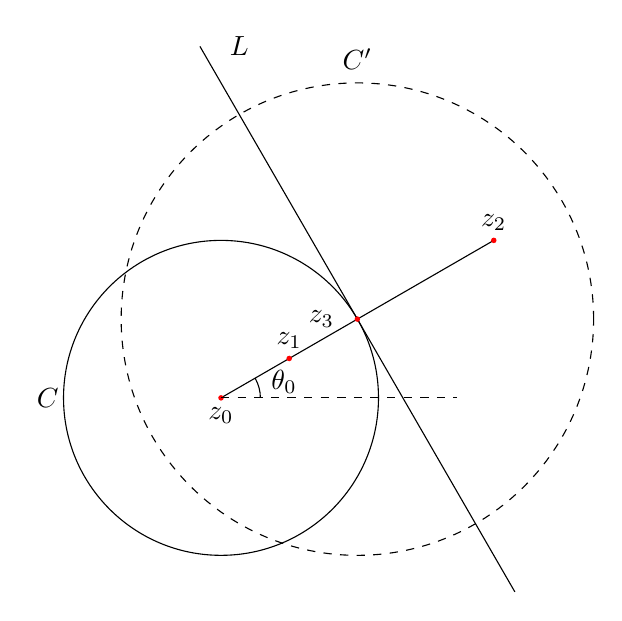
\begin{tikzpicture}
    \draw (0,0) circle [radius = 2cm];
    \coordinate [label= below:$z_0$](Z) at (0,0);
    \coordinate [label = above:$z_1$](Z1) at(30:1);
    \coordinate [label = 90:$z_2$](Z2) at (30:4);
    \coordinate [](Z3) at (30:2);
    \node[xshift = -13pt] at (Z3){$z_3$};
    \draw (Z)--(Z1)--(Z2); 
    \draw (Z3)++(120:4cm) coordinate(L)--(Z3);
    \draw (Z3)++(-60:4cm)--(Z3);
    \draw[dashed] (Z3) circle [radius = 3cm];
    \draw (Z3)++(90:3)coordinate(C');
    \node[yshift = 2ex] at (C'){$C'$};
    \node[xshift = .5cm] at(L){$L$};
    \node[xshift = -2.2cm]at (Z){$C$};
    \fill[red] (Z) circle (1pt);
    \fill[red] (Z1) circle (1pt);
    \fill[red] (Z2) circle (1pt);
    \fill[red] (Z3) circle (1pt);
    \draw[dashed] (Z)--(3,0)coordinate (A);
    \draw(5mm,0) arc [start angle = 0, end angle = 30, radius = 5mm];
    \node[xshift = .8cm, yshift = .2cm] (0,0){$\theta_0$};
    \end{tikzpicture}
    \caption{问题2解法1示意图}
    \label{fig:2}
    \end{wrapfigure}
    \noindent 两边取模,则有
    $$|z-z_3|=k$$
    则
    \begin{equation*}\begin{split}
        \left|z-z_3\right|^2 &=(z-z_3)(\overline{z-z_3})=kie^{i\theta_0}(\overline{z-z_3})\\&=\left|z-z_3\right|ie^{i\theta_0}(\overline{z-z_3})
    \end{split}
\end{equation*}
    即
    $$
    \left|z-z_3\right|=ie^{i\theta_0 }(\overline{z-z_3})=k
    $$
    代入式~\eqref{equ:line}~中,得到直线$L'$表达式:
    $$
    z-z_3=ie^{i\theta_0}(\overline{z-z_3})ie^{i\theta_0}
    $$
    整理后得到:
    \begin{equation}
    (z-z_3)e^{-i\theta_0}+(\overline{z-z_3})e^{i\theta_0}=0
    \label{equ:L'}
    \end{equation}
    为$L'$的方程。
    

    下面求解圆$C$的方程。其一般形式应该为式~\eqref{equ:circle}~:
    \begin{equation*}
    z\bar{z}+\bar{\alpha}z+\alpha \bar{z}+\beta=0
    \end{equation*}对应的圆心和半径为:
    \begin{equation*}
    \begin{cases}
    z_0=-\alpha\\
    r=\sqrt[]{|\alpha|^2-\beta}
    \end{cases}
    \end{equation*}
    将$\alpha$和$\beta$用$z_0$和$r$表示后代入式~\eqref{equ:circle}~中可得:
    \begin{equation*}
    z\bar{z}-\overline{z_0}z-z_0 \bar{z}+|z_0|^2-r^2=0
    \end{equation*}
    又有$z_3=z_0+re^{i\theta}$,则
    \begin{equation*}
    z\bar{z}-(\overline{z_3-re^{i\theta}})z-(z_3-re^{i\theta}) \bar{z}+|z_3-re^{i\theta}|^2-r^2=0
    \end{equation*}
    或
    \begin{equation*}
    z\bar{z}-(\overline{z_3-re^{i\theta}})z-(z_3-re^{i\theta}) \bar{z}+(z_3-re^{i\theta})(\overline{z_3-re^{i\theta}})-r^2=0
    \end{equation*}
    最终化简为
    \begin{equation}
    (z-z_3)e^{-i\theta_0}+(\overline{z-z_3})e^{i\theta_0}=\dfrac{\overline{z_3}z+z_3\bar{z}-|z_3|^2-|z|^2}{r}
    \label{circle2}
    \end{equation}
    不难看出,式~\eqref{equ:L'}~和式~\eqref{circle2}~十分接近。下面证明当$r\rightarrow\infty$时,$C$趋近于直线$L'$。
    以$z_3$为圆心,$R$为半径作圆$C'$。设圆$C$上在圆$C'$内的部分为$Arc$,其上的任一点$\xi $,必有$$|\xi|=|\xi-z_3+z_3|\le |\xi-z_3|+|z_3|\le R+|z_3|$$由已经假定$z_3$不动,故$|z_3|$有界,因此$\exists M_1>0,s.t. |z_3|<M_1$。则$\exists M_2 =M_1+R,s.t. |\xi|<M_2$
    
    不难证明,复平面上任意一点$\omega$到直线$\bar{\alpha}z+\alpha \bar{z}+\beta=0$的距离为
    \begin{equation}
    \frac{|\bar{\alpha}z+\alpha \bar{z}+\beta|}{2|\alpha|}
    \end{equation}
    则$\xi$点到$L'$的距离为
    \begin{equation}
    d=\frac{|(\xi-z_3)e^{-i\theta_0}+(\overline{\xi-z_3})e^{i\theta_0}|}{2}
    \end{equation}
    注意到点$\xi$在$C$上,则有
    \begin{equation}
    (\xi-z_3)e^{-i\theta_0}+(\overline{\xi-z_3})e^{i\theta_0}=\dfrac{\overline{z_3}\xi+z_3\bar{\xi}-|z_3|^2-|\xi|^2}{r}
    \end{equation}
    则
    \begin{equation}
    \begin{split}
    d&=\dfrac{|\overline{z_3}\xi+z_3\bar{\xi}-|z_3|^2-|\xi|^2|}{2r}\\
    &\le\dfrac{|\overline{z_3}\xi|+|z_3\bar{\xi}|+|z_3|^2+|\xi|^2}{2r}\\
    &\le \dfrac{M_1M_2+M_1M_2+M_1^2+M_2^2}{2r}\\
    &=\dfrac{(M_1+M_2)^2}{2r}
    \end{split}
    \end{equation}
    则$\forall \varepsilon >0,\exists r_1 = \frac{(M_1+M_2)^2}{2\varepsilon}+1$,使得$\forall r>r_1,\xi \in Arc$,均有$d<\varepsilon$。则可知圆$C$在圆$C'$内的部分($Arc$)在$r\rightarrow\infty$时趋于直线$L'$。另一方面,由于$C'$的半径是任意选取的,故得出结论:圆$C$在$r\rightarrow\infty$时趋于直线$L'$。即待求$L$和$L'$重合。
    
    既然$L'$即为待求直线,而$L'$又是圆的切线,则自然有$L'\bot \overline{z_0z_1}$,或$L\bot \overline{z_0z_1}$成立。命题1得证。\hfill $\square$
    
    下面证明命题2。由于$z_2$和$z_1$是关于圆$C$的对称点,故有
    \begin{equation}
    z_2=z_0+\frac{r^2}{\overline{z_1-z_0}}
    \end{equation}
    由命题1的证明可以看出,$r\rightarrow\infty$时圆$C$趋于直线$L$,且直线$L$即为在$z_3$处的切线。设$d_1=|z_3-z_1|,d_2=|z_3-z_2|$
    由于$z_0,z_1,z_2,z_3$四点共线,故有
    \begin{equation}
    \begin{cases}
    z_1=z_0+r_1e^{i\theta_0}\\
    z_2=z_0+r_2e^{i\theta_0}\\
    z_3=z_0+re^{i\theta_0}
    \end{cases}
    \end{equation}
    故有
    \newcommand{\ei}{e^{i\theta_0}}
    \begin{equation}
    \begin{split}
    \dfrac{d_2}{d_1}&=\dfrac{r_2-r}{r-r_1}=\dfrac{\dfrac{z_2-z_3}{e^{i\theta_0}}}{\dfrac{z_3-z_1}{e^{i\theta_0}}}=\dfrac{z_2-z_3}{z_3-z_1}=\dfrac{z_0+\dfrac{r^2}{\overline{z_1-z_0}}-z_3}{z_3-z_1}\\
    &=\dfrac{-r\ei+\dfrac{r^2}{\overline{r_1\ei}}}{(r-r_1)\ei}=\dfrac{-r\ei+\dfrac{r^2}{r_1e^{-i\theta_0}}}{(r-r_1)\ei}\\
    &=\dfrac{-r+\dfrac{r^2}{r_1}}{r-r_1}=\dfrac{\dfrac{r(r-r_1)}{r_1}}{r-r_1}\\
    &=\dfrac{r}{r_1}=\dfrac{r}{r-d_1}
    \end{split}
    \end{equation}
    其中$d_1$为定值,则显然有
    \begin{equation}
    \lim_{r\rightarrow\infty} \dfrac{d_2}{d_1}=1
    \end{equation}
    即$r\rightarrow\infty$时$d_1=d_2$,证毕。
    \end{SOLUTION}
    \begin{SOLUTION}[法2]
    事实上,本题中要求证明的结论都是几何关系,只与点之间的相对位置有关,故可以通过坐标变换简化。本题中的$z_0,z_1,z_2,z_3$均共线,故先将图形旋转使得$z_0,z_1,z_1,z_3$所在直线与实轴平行,再整体平移使得$z_3$与原点重合。由于平移变换与旋转变换不改变垂直关系和距离大小,故这样的变换是合理的。
    
    \begin{wrapfigure}[18]{R}{0.5\textwidth}
    \begin{tikzpicture}
    \draw[->,>=stealth] (-5,0)--(4,0) node[below] {$x$};
    \draw (0,-3)--(0,3) node[right] (L){$L$};
    \draw[name path = circle] (-2,0) circle [radius = 2];
    \draw (0,0) node[right = .5cm, below] (O){$O(z_3)$};
    \draw (-2, 0) node[below] (z0){$z_0$};
    \node at (-4,-1.5) {$C$};
    \draw (-1, 0) node[below] (z1){$z_1$};
    \draw (3, 0) node[below] (z2){$z_2$};
    \fill[red] (0,0) circle [radius = 1pt];
    \fill[red] (-2,0) circle [radius = 1pt];
    \fill[red] (-1,0) circle [radius = 1pt];
    \fill[red] (3,0) circle [radius = 1pt];
    \path[name path = line](0,0)--(130:5);
    \draw[name intersections={of = line and circle}] (intersection-2)coordinate (B) --node[above]{$\rho$}(0,0);
    \draw (3mm, 0) arc [start angle = 0, end angle = 130, radius = 3mm];
    \node[above=.3cm,right=.3cm] (0,0) {$\theta$};
    \fill[red] (B) circle[radius = 1pt];
    \draw[dashed] (0,0) let
    \p1 = ($ (0,0) - (B) $)
    in
    circle ({veclen(\x1,\y1)});
    \draw[red,thick] let \p1 = ($(0,0)-(B)$) in (B)--node[above, color = red]{$d$}(0,-\y1)coordinate(E);
    \node at (2,2) {$C'$};
 
 
    \end{tikzpicture}
    \caption{问题2解法2示意图}
    \label{fig:q2s2}
    \end{wrapfigure}
    
    如图~\ref{fig:q2s2}~所示,经过平移和旋转变换后,可以在极坐标下求解。仍固定$z_3$和$z_1$。此时圆$C$的极坐标方程为
    \begin{equation}
    \rho = -2r\cos \theta
    \end{equation}
    其中$r$为圆$c$的半径。图中$L$为圆$C$在原点处的切线,下面证明当$r\rightarrow\infty$时圆$C$的极限就是$L$。
    
    仍记圆$C$在单位圆$\rho=R$中的部分为$Arc$。不难得出出$Arc$上的点到直线$L$的距离为
    $d=\rho\cos(\pi-\theta)=-\rho\cos\theta$。而当$\rho=R$(图中所示情况)时,$d$有最大值$d_{\max}=-R\cos\theta$。下面固定$\rho=R$不变,改变$r$的大小,则有
    $$d_{\max}=-R\cdot \frac{\rho}{-2r}=\frac{R^2}{2r}$$
    则$\forall \varepsilon>0,\exists r_1 = \max\left\{\dfrac{R^2}{2\varepsilon},\dfrac{R}{2}\right\},s.t$当$r>r_1$时$Arc$上的所有点到$L$的距离都满足$d\le d_{\max}<\varepsilon$,则$Arc$在$r\rightarrow \infty$时趋于$L$。另一方面,由于$R$可以任意取,则圆$C$在$r\rightarrow\infty$时趋于$L$。且由于$L$为$C$在原点处的切线,显然有$L\bot\overline{z_0z_1}$,命题1得证。\hfill$\square$
    
    下面证明命题2。设$z_1$和$z_2$到直线$L$的距离分别为$d_1,d_2$。事实上,$d_1=|z_1|,d_2=|z_2|$。由$z_1$和$z_2$关于圆$C$对称的定义,可知:
    \begin{equation}
    |z_0|^2=|z_1-z_0|\cdot|z_2-z_0|
    \end{equation}
    或
    \begin{equation}
    r^2=(r-d_1)(r+d_2)
    \label{equ:rd12}
    \end{equation}
    由式~\eqref{equ:rd12}~立得:
    \begin{equation*}
    r^2=r^2+r(d_2-d_1)-d_1d_2
    \end{equation*}
    进一步有
    \begin{equation}
    \dfrac{d_1}{d_2}=1-\dfrac{d_1}{r}
    \end{equation}
    由于假定$z_1$固定,则$d_1$为定值,故对上式令$r\rightarrow\infty$可得$\lim_{r\rightarrow\infty}\limits\dfrac{d_1}{d_2}=1$。即当$r\rightarrow\infty$时,$z_1$和$z_2$到$L$的距离相等。命题2得证。
    \end{SOLUTION}
    \begin{QUESTION}
    求单值解析映射$\omega=\omega(z)$将异心圆环之间部分映成同心圆环之间部分,且使内环或外环半径为1.
    \end{QUESTION}
    \begin{SOLUTION}
    不妨先考虑将异心圆环之间部分映成单位同心圆环的分式线性映射。
    \begin{figure}
        \begin{center}
        \subfigure[异心圆环]
        {
        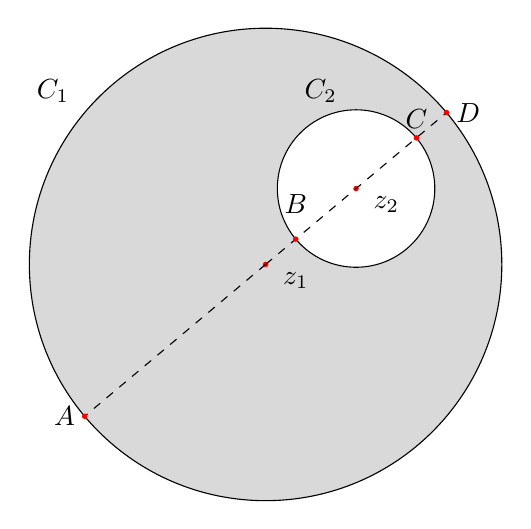
\begin{tikzpicture}
        \fill [color = black!15!white] (0,0) circle (3);
        \filldraw[color=white](40:1.5) circle (1);
        \draw (0,0) coordinate (Z1) node[below = .2cm, right = .1cm] {$z_1$}circle (3);
        \draw (0,0)++(40:1.5)coordinate (Z2) node[below = .2cm, right = .1cm] {$z_2$}circle (1);
        \fill[red] (Z1) circle[radius = 1pt];
        \fill[red] (Z2) circle[radius = 1pt];
        \draw[dashed] (Z1)--++(220:3) coordinate (A);
    
        \draw[dashed] (Z1)--(40:0.5)coordinate(B) --(40:2.5) coordinate (C)--(40:3) coordinate (D);
        \fill[red] (A) circle[radius = 1pt];
        \fill[red] (B) circle[radius = 1pt];
        \fill[red] (C) circle[radius = 1pt];
        \fill[red] (D) circle[radius = 1pt];
        
        \node[below, left] at (A){$A$};
        \node[above] at (C){$C$};
        \node[above = .2cm] at (B){$B$};
        \node[above, right] at (D){$D$};
        \node at (.7,2.2){$C_2$};
        \node at (-2.7,2.2){$C_1$};
        \end{tikzpicture}
        \label{fig:3z}
        }
        \hspace{2cm}
        \subfigure[同心圆环]
        {
        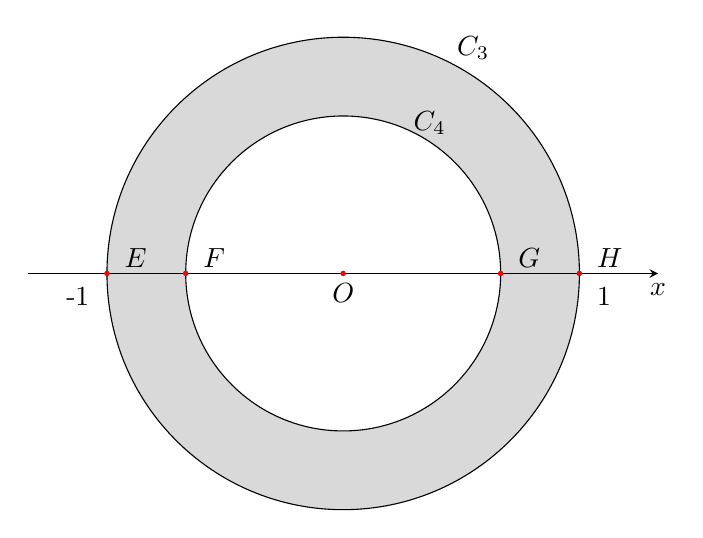
\begin{tikzpicture}
        \fill[color = black!15] (0,0) circle (3);
        \fill[color = white] (0,0) circle (2);
        \draw (0,0) node[below] {$O$}  circle (3);
        \draw[->, >=stealth](-4, 0)--(4,0) node[below]{$x$};
        \node [below=.3cm, left = .1cm] at (-3, 0) {-1};
        \node [below = .3cm, right = .1cm] at (3, 0) {1};
        \draw circle(2);
        \fill[red] (-3,0) circle[radius = 1pt];
        \fill[red] (3,0) circle[radius = 1pt];
        \fill[red] (0,0) circle[radius = 1pt];
        \fill[red] (2,0) circle[radius = 1pt];
        \fill[red] (-2,0) circle[radius = 1pt];
        \node[above=.2cm, right = .1cm] at (-3, 0) {$E$};
        \node[above=.2cm, right = .1cm] at (-2, 0) {$F$};
        \node[above=.2cm, right = .1cm] at (2, 0) {$G$};
        \node[above=.2cm, right = .1cm] at (3, 0) {$H$};
        \node at (60:2.2) {$C_4$};
        \node at (60:3.3) {$C_3$};
        \end{tikzpicture}
        \label{fig:3w}
        }
        \end{center}
        \caption{思考题3示意图}
        \label{fig:3}
    \end{figure}
    如图~\ref{fig:3}~所示。设两个异心圆$C_1,C_2$的圆心分别为$z_1$和$z_2$,对应的半径分别为$r_1$和$r_2$,圆心距为$d=|z_1-z_2|$。设过$z_1$和$z_2$的直线与两个圆依次交于$A,B,C,D$四个点。设$\arg (z_2-z_1)=\theta_0$。现考虑分式线性变换$T_1(z)$
    \begin{equation}
    T_1(z)=k\frac{z-A}{z-D}
    \label{equ:3z'}
    \end{equation}
    其中$k\in\mathbb{C}$为待定常数。记$T_1(z)$的像为$z'$。则显然式~\ref{equ:3z'}~将$A$映到原点,将$D$映到$\infty$。即$A'=0,D'=\infty$。由于分式线性变换保广义圆,故经变换后$C_1$变为一条直线,记做$L_1'$。将$B$点代入,计算可得:
    \begin{equation}
        B'=k\frac{B-A}{B-D}=k\frac{|B-A|e^{i\theta_0}}{-|D-B|e^{i\theta_0}}=-k\dfrac{|B-A|}{|D-B|}=-k\dfrac{r_1+d-r_2}{r_1-d+r_2}
        \label{equ:B'}
    \end{equation}
    若取$k$为负实数,则可以保证$B'$位于正实轴。由于分式线性变换保广义圆,且$A,B,C,D$四点共线,则$A'B'C'D'$四点共广义圆;而又由$A'$和$B'$都位于实轴,故直线$AB$经过式~\ref{equ:3z'}~映射后仍为直线,且为实轴。另一方面,由于分式线性变换具有保角性,故直线$AD$和圆$C_1$在$A$处的夹角经过映射之后保持不变,即也为90\textdegree。综上,圆$C_1$经过映射后变为直线$L'$,且$L'\bot A'B'$。进而得出$L'$和虚轴重合。
    
    同理不难得出
    \begin{equation}
    C'=k\dfrac{C-A}{C-D}=-k\dfrac{r_1+r_2+d}{r_1-r_2-d}
    \label{equ:C'}
    \end{equation}
    也位于正实轴上。考虑函数
    $$y=\dfrac{2r_1+x-r_1}{r_1-x}=\dfrac{2r_1}{r_1-x}-1$$易知当$x<r_1$时$y$为单调增函数。注意到$d-r_2<d+r_2<r_1$,故有
    $$
    \dfrac{r_1+(r_2+d)}{r_1-(r_2+d)}>\dfrac{r_1+(d-r_2)}{r_1-(d-r_2)}
    $$
    即$C'>B'$。则$T_1$将圆$C_2$映成过点$B',C'$的圆。又由分式线性变换的保角性,且圆$C_2$与直线$BC$在$B$处切线夹角为90\textdegree,则圆$C_2'$与直线$B'C'$的切线在$B'$处的夹角也为90\textdegree,即$B'C'$为圆$C_2'$的直径。这样,我们证明了$T_1$可以将圆$C_1$和$C_2$分别映成直线(虚轴)和位于右半平面且圆心在实轴的圆。如图~\ref{fig:3z'}~所示。进一步地,我们需要证明$T_1$将图~\ref{fig:3z}~中的阴影部分映成图~\ref{fig:3z'}~中的阴影部分。首先考虑圆$C_1$内部的任何一点$z$,则必有$\angle AzD>90^\circ$。由此可以得出:
    \begin{equation}
        \arg \left(\dfrac{z-A}{z-D}\right)\in \left(\frac{\pi}{2},\frac{3\pi}{2}\right)
    \end{equation}
    即$\arg z'\in(-\frac{\pi}{2},\frac{\pi}{2})$,故${\rm Re} z'>0$。即$T_1$将$C_1$内部的点映成右半平面的点,同理将$C_1$外部的点映成左半平面的点。对于圆$C_2$外部的点$z$,有$\angle BzC<90^\circ$,或
    \begin{equation}
        \arg\left(\dfrac{z-B}{z-C}\right)\in \left(-\dfrac{\pi}{2},0\right)\cup\left(0, \dfrac{\pi}{2}\right)
    \end{equation}
    而
    \begin{equation}
        \begin{split}
            \arg\left(\dfrac{z'-B'}{z'-C'}\right)&=\arg\left(\dfrac{k\dfrac{z-A}{z-D}-k\dfrac{B-A}{B-D}}{k\dfrac{z-A}{z-D}-k\dfrac{C-A}{C-D}}\right)\\
            &=\arg\left(\dfrac{\dfrac{zB-zD-AB+AD-zB+BD+Az-AD}{(z-D)(B-D)}}{\dfrac{zC-zD-AC+AD-zC+CD+Az-AD}{(z-D)(C-D)}}\right)\\
            &=\arg\left(\dfrac{\dfrac{-zD-AB+BD+Az}{(z-D)(B-D)}}{\dfrac{-zD-AC+CD+Az}{(z-D)(C-D)}}\right)=\arg\left(\dfrac{\dfrac{(A-D)(z-B)}{(z-D)(B-D)}}{\dfrac{(A-D)(z-C)}{(z-D)(C-D)}}\right)\\
            &=\
            arg\left(\dfrac{z-B}{z-C}\cdot\dfrac{C-D}{B-D}\right)=\arg\left(\dfrac{z-B}{z-C}\right)+\arg\left(\dfrac{C-D}{B-D}\right)\\
            &=\arg\left(\dfrac{C-D}{B-D}\right)\in  \left(-\dfrac{\pi}{2},0\right)\cup\left(0, \dfrac{\pi}{2}\right)
        \end{split}
    \end{equation}
    上式中利用了$\frac{C-D}{B-D}$为正实数这一事实。这样,我们证明了$T_1$将$C_2$外部的点映成$C_2'$外部的点。同理$T_1$将$C_2$内部的点映成$C_2'$内部的点。进而可以得出,$T_1$将图~\ref{fig:3z}~中的阴影部分映成图~\ref{fig:3z'}~中的阴影部分。
    \begin{figure}
    \begin{center}
    \subfigure[异心圆环经$T_1$映射]
    {
    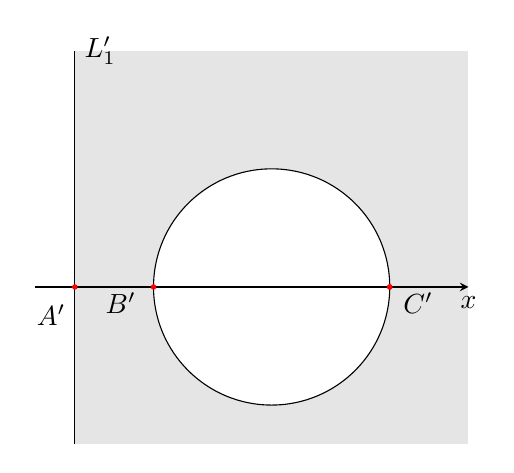
\begin{tikzpicture}
    \fill[color = black!10!white] (-0.5,-2) rectangle (4.5, 3);
    \fill[color = white] (2,0) circle (1.5);
    \draw[->,>=stealth] (-1, 0)--(4.5,0)node[below]{$x$};
    \draw (-0.5,-2)--(-0.5,3)node[right]{$L_1'$};
    \draw (2,0) circle (1.5);
    \node[below=.2cm, left = .1cm] at (0.5,0){$B'$};
    \node[left = .3cm, below = .1cm] at (-0.5,0){$A'$};
    \node[below=.2cm, right = .05cm] at (3.5,0) {$C'$};
    \fill[red] (0.5,0) circle[radius = 1pt];
    \fill[red] (-0.5,0) circle[radius = 1pt];    
    \fill[red] (3.5,0) circle[radius = 1pt];
    \fill[red] (3.5,0) circle[radius = 1pt];
    \end{tikzpicture}
    \label{fig:3z'}
    }
    \hspace{1cm}
    \subfigure[同心圆环经$T_2$映射]
    {
    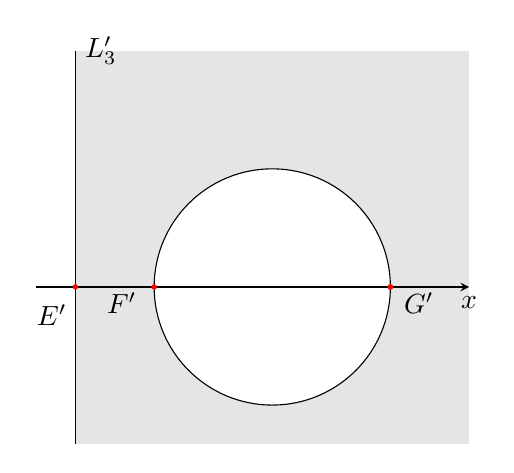
\begin{tikzpicture}
    \fill[color = black!10!white] (-0.5,-2) rectangle (4.5, 3);
    \fill[color = white] (2,0) circle (1.5);
    \draw[->,>=stealth] (-1, 0)--(4.5,0)node[below]{$x$};
    \draw (-0.5,-2)--(-0.5,3)node[right]{$L_3'$};
    \draw (2,0) circle (1.5);
    \node[below=.2cm, left = .1cm] at (0.5,0){$F'$};
    \node[left = .3cm, below = .1cm] at (-0.5,0){$E'$};
    \node[below=.2cm, right = .05cm] at (3.5,0) {$G'$};
    \fill[red] (0.5,0) circle[radius = 1pt];
    \fill[red] (-0.5,0) circle[radius = 1pt]; 
    \fill[red] (3.5,0) circle[radius = 1pt];
    \fill[red] (3.5,0) circle[radius = 1pt];
    \end{tikzpicture}
    \label{fig:3w'}
    }
    \end{center}
    \caption{经分式线性变换$T_1,T_2$后示意图}
    \label{fig:aftermap}
    \end{figure}
    先假定目标同心圆的外径为1,两个圆记做$C_3$和$C_4$,半径分别为$r_3,r_4$。实轴在水平方向上依次交两个圆于$E,F,G,H$四个点。对同心圆环,同理做分式线性变换$T_2(\omega)$:
    \begin{equation}
        T_2(\omega)=l\frac{\omega-E}{\omega-H}
        \label{equ:3w'}
    \end{equation}
   
    其中$l\in\mathbb{C}$。记$T_2(\omega)$的像为$\omega'$。
    则类似地,若令$l$为负实数,则有$E'=0$,$H'=\infty$。$C_3$经过映射后变为垂直于实轴的直线$L_3'$,且$F',G'$均在正实轴上。并有
    \begin{equation}
    \begin{cases}
    F'=l\dfrac{F-E}{F-H}=-l\dfrac{r_3-r_4}{r_3+r_4}\\[2ex]
    G'=l\dfrac{G-E}{G-H}=-l\dfrac{r_3+r_4}{r_3-r_4}
    \end{cases}
    \end{equation}
    且同理可证$T_2$将图~\ref{fig:3w}~中的阴影部分映成图~\ref{fig:3w'}~中的阴影部分。
    从图~\ref{fig:aftermap}~中可以看到,原始的异心圆环与目标的同心圆环分别经过$T_1(z)$和$T_2(\omega)$的映射后的图形十分相似。故可以通过调整$k$和$l$的取值,从而在图~\ref{fig:3z'}~和图~\ref{fig:3w'}~中建立联系,使得$z'$和$\omega'$表示的区域相同。
    令$B'=F',C'=G'$可得:
    \begin{equation}
    \begin{cases}
    -k\dfrac{r_1+d-r_2}{r_1-d+r_2}=-l\dfrac{r_3-r_4}{r_3+r_4}\\[2ex]
    -k\dfrac{r_1+r_2+d}{r_1-r_2-d}=-l\dfrac{r_3+r_4}{r_3-r_4}
    \end{cases}
    \end{equation}
    上述两个方程相乘再开根号(注意到$k<0,l<0$),即可得到:
    \begin{equation}
        k\sqrt{\dfrac{r_1+d-r_2}{r_1-d+r_2}\cdot\dfrac{r_1+r_2+d}{r_1-r_2-d}}=l
    \end{equation}
    由$T_2(\omega)$的表达式~\eqref{equ:3w'}~,将$E=-1,H=1$代入,即有
    $$
    \omega'=l\dfrac{\omega+1}{\omega-1}
    $$
    从中将$\omega$反解出来,即有:
    \begin{equation}
        \omega = \dfrac{\omega'+l}{\omega'-l}
    \end{equation}
    即为$T^{-1}_2$的表达式。
    记$$\begin{cases}
        \alpha = \sqrt{\dfrac{r_1+d-r_2}{r_1-d+r_2}}\\[2ex]
        \beta = \sqrt{\dfrac{r_1+r_2+d}{r_1-r_2-d}}
    \end{cases}$$
    则$l=k\alpha\beta$,可以写出$\omega$与$z$的关系式如下:
    \begin{equation}
        \begin{split}
        \omega &= \dfrac{\omega'+l}{\omega'-l}=\dfrac{z'+l}{z'-l}\\
        &= \dfrac{k\dfrac{z-A}{z-D}+l}{k\dfrac{z-A}{z-D}-l}\\&=\dfrac{k(z-A)+k\alpha\beta(z-D)}{k(z-A)-k\alpha \beta(z-D)}\\
        &=\dfrac{(z-A)+\alpha\beta(z-D)}{(z-A)-\alpha\beta(z-D)}
        \end{split}
    \end{equation}
    将$\alpha$和$\beta$的值代入,即可得到所求表达式:
    \begin{equation}
        \omega(z)=\dfrac{(z-A)+\sqrt{\dfrac{r_1+d-r_2}{r_1-d+r_2}\cdot\dfrac{r_1+r_2+d}{r_1-r_2-d}}(z-D)}{(z-A)-\sqrt{\dfrac{r_1+d-r_2}{r_1-d+r_2}\cdot\dfrac{r_1+r_2+d}{r_1-r_2-d}}(z-D)}
        \label{equ:3final}
    \end{equation}

    事实上,上述构造的过程中已经保证了式~\eqref{equ:3final}~的正确性。且由于分式线性映射必为单值解析映射,故自然满足题中条件。下面对式~\eqref{equ:3final}~进行进一步的讨论。从中不难看出$\omega(A)=-1$而$\omega(D)=1$。另一方面由式~\eqref{equ:B'}~可知,
    $$
    \dfrac{B-A}{B-D}=-\dfrac{r_1+d-r_2}{r_1-d+r_2}=-\alpha^2
    $$
    同理由式~\eqref{equ:C'}~有
    $$
    \dfrac{C-A}{C-D}=-\dfrac{r_1+r_2+d}{r_1-r_2-d}=-\beta^2
    $$
    可以求得:
    \begin{equation}
        \begin{cases}
            \omega(B)=\dfrac{\dfrac{B-A}{B-D}+\alpha\beta}{\dfrac{B-A}{B-D}-\alpha\beta}=\dfrac{-\alpha^2+\alpha\beta}{-\alpha^2-\alpha\beta}=\dfrac{\alpha-\beta}{\alpha+\beta}\\[3ex]
            \omega(C)=\dfrac{\dfrac{C-A}{C-D}+\alpha\beta}{\dfrac{C-A}{C-D}-\alpha\beta}=\dfrac{-\beta^2+\alpha\beta}{-\beta^2-\alpha\beta}=\dfrac{\beta-\alpha}{\alpha+\beta}
        \end{cases}
    \end{equation}
    可知$\omega(z)$将$B$和$C$映射成实轴上关于原点对称的两点,且显然有$|\omega(B)|=|\omega(C)|<1$。考虑使式~\eqref{equ:3final}~分母为零的点$z_0$,必有
    $$
    \dfrac{z_0-A}{z_0-D}=\alpha\beta\in\mathbb{R}
    $$
    则说明$z_0$必然在直线$AD$上,则圆$C_1$和$C_2$上的任何一点都不会被映成无穷远点($\omega(A),\omega(B),\omega(C),\omega(D)$已经求出,不是$\infty$),所以圆$C_1$和$C_2$经过映射后仍为圆。显然$\omega(z)$将直线$AD$映成直线$EH$。由于分式线性变换保角,且圆$C_1$在$A$处切线垂直于$AD$,故映射后$C_3$在$E$处切线垂直于$EH$,即$EH$是圆$C_3$的直径,同理$FG$是圆$C_4$的直径,满足要求。

    一般地,如果同心圆盘的圆心不在原点,不妨设为$\omega_0$,则只需在式~\eqref{equ:3final}~后面加上$\omega_0$即可:
    \begin{equation}
        \tag{\ref{equ:3final}$'$}
        \omega_1(z)=\dfrac{(z-A)+\sqrt{\dfrac{r_1+d-r_2}{r_1-d+r_2}\cdot\dfrac{r_1+r_2+d}{r_1-r_2-d}}(z-D)}{(z-A)-\sqrt{\dfrac{r_1+d-r_2}{r_1-d+r_2}\cdot\dfrac{r_1+r_2+d}{r_1-r_2-d}}(z-D)}+\omega_0
        \label{equ:3final+1}
    \end{equation}
    
    \hfill $\square$

   上述过程已经构造出将异心圆盘映成外径为1的同心圆盘的分式线性映射。事实上,将异心圆盘其映成内径为1的同心圆盘的原理类似。只需令
    \begin{equation}
        \begin{cases}
        \hat{T}_1(z)=\hat{k}\dfrac{z-B}{z-C}\\
        
        \hat{T}_2(\omega)=\hat{l}\dfrac{\omega-F}{\omega-G}
    \end{cases}
    \end{equation}
    此时同理可证,$\hat{T_1}$和$\hat{T_2}$分别将异心圆环域和同心圆环域映成图~\ref{fig:3zz'}~和图~\ref{fig:3ww'}~。此时$\hat{k}$和$\hat{l}$取正实数。
    \begin{figure}[!htb]
        \begin{center}
        \subfigure[异心圆环经$\hat{T}_1$映射]
        {
        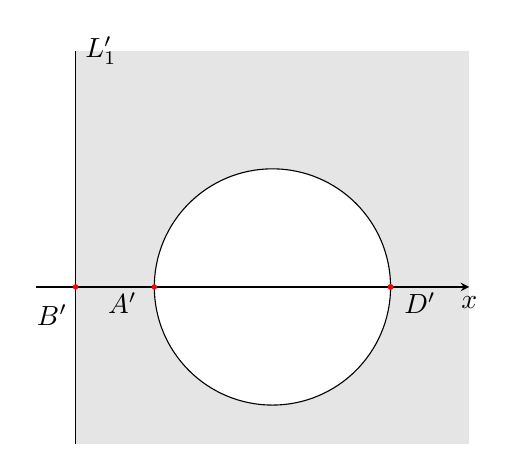
\begin{tikzpicture}
        \fill[color = black!10!white] (-0.5,-2) rectangle (4.5, 3);
        \fill[color = white] (2,0) circle (1.5);
        \draw[->,>=stealth] (-1, 0)--(4.5,0)node[below]{$x$};
        \draw (-0.5,-2)--(-0.5,3)node[right]{$L_1'$};
        \draw (2,0) circle (1.5);
        \node[below=.2cm, left = .1cm] at (0.5,0){$A'$};
        \node[left = .3cm, below = .1cm] at (-0.5,0){$B'$};
        \node[below=.2cm, right = .05cm] at (3.5,0) {$D'$};
        \fill[red] (0.5,0) circle[radius = 1pt];
        \fill[red] (-0.5,0) circle[radius = 1pt];    
        \fill[red] (3.5,0) circle[radius = 1pt];
        \fill[red] (3.5,0) circle[radius = 1pt];
        \end{tikzpicture}
        \label{fig:3zz'}
        }
        \hspace{1cm}
        \subfigure[同心圆环经$\hat{T}_2$映射]
        {
        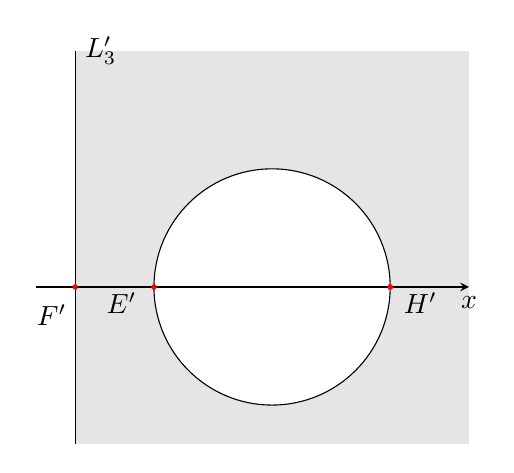
\begin{tikzpicture}
        \fill[color = black!10!white] (-0.5,-2) rectangle (4.5, 3);
        \fill[color = white] (2,0) circle (1.5);
        \draw[->,>=stealth] (-1, 0)--(4.5,0)node[below]{$x$};
        \draw (-0.5,-2)--(-0.5,3)node[right]{$L_3'$};
        \draw (2,0) circle (1.5);
        \node[below=.2cm, left = .1cm] at (0.5,0){$E'$};
        \node[left = .3cm, below = .1cm] at (-0.5,0){$F'$};
        \node[below=.2cm, right = .05cm] at (3.5,0) {$H'$};
        \fill[red] (0.5,0) circle[radius = 1pt];
        \fill[red] (-0.5,0) circle[radius = 1pt]; 
        \fill[red] (3.5,0) circle[radius = 1pt];
        \fill[red] (3.5,0) circle[radius = 1pt];
        \end{tikzpicture}
        \label{fig:3ww'}
        }
        \end{center}
        \caption{经分式线性变换$\hat{T}_1,\hat{T}_2$后示意图}
        \label{fig:hat}
        \end{figure}
        使用类似的推导方式,可以得出$\hat{\omega}(z)$的表达式(详细过程从略)。设
        \begin{equation}
            \begin{cases}
                \hat{\alpha} = \sqrt{\dfrac{r_1+d-r_2}{r_1+d+r_2}}\\
                \hat{\beta} = \sqrt{\dfrac{r_1-d+r_2}{r_1-d-r_2}}
            \end{cases}
        \end{equation}
        则
        \newcommand{\halpha}{\hat{\alpha}}
        \newcommand{\hbeta}{\hat{\beta}}
        \begin{equation}
            \hat{\omega}(z)=\dfrac{(z-B)+\hat{\alpha}\hat{\beta}(z-C)}{(z-B)-\halpha\hbeta(z-C)}
            \label{equ:final_hat}
        \end{equation}
        且有
        $$
        \begin{cases}
            \hat{\omega}(A)=\dfrac{\halpha+\hbeta}{\halpha-\hbeta}\\
            \hat{\omega}(B)=\dfrac{\halpha+\hbeta}{\hbeta-\halpha}
        \end{cases}
        $$
        一般地,若要求目标的同心圆盘中心位于$\omega_0$,则有
        \begin{equation}
            \tag{\ref{equ:final_hat}$'$}
            \hat{\omega}_1(z)=\dfrac{(z-B)+\halpha\hbeta(z-C)}{(z-B)-\halpha\hbeta(z-C)}+\omega_0
        \end{equation}
\end{SOLUTION}
    \end{document}
    